% !TeX root = ../main.tex

\chapter{个人贡献}

在此次大作业中,我负责编写测试所需的 Shell 脚本、实现函数图像的绘制工作。为了便于组内其他成员进行性能对比图像的绘制,测试所用的 Shell 脚本将以 Python 数组的形式进行输出,以便于图像数据的读入。在函数图像的绘制部分,我在组内其他成员的工作基础上通过 Python 语言使用 matplotlib 绘图库绘制了所求函数和所求函数的次梯度函数的图像。

\paragraph{测试脚本}

由组内其他成员编写的 C 语言求解程序,通过读取 madbc.txt 文件作为数据的输入。因而我们的测试脚本通过生成测试数据并写入 madbc.txt 来进行对两个算法程序的测试。为了生成测试数据,我们通过编写 Python 程序并由 Shell 脚本进行调用,用于生成测试数据的 Python 脚本如图 (\ref{Python}) 所示。
\begin{figure}[htb]
    \centering
    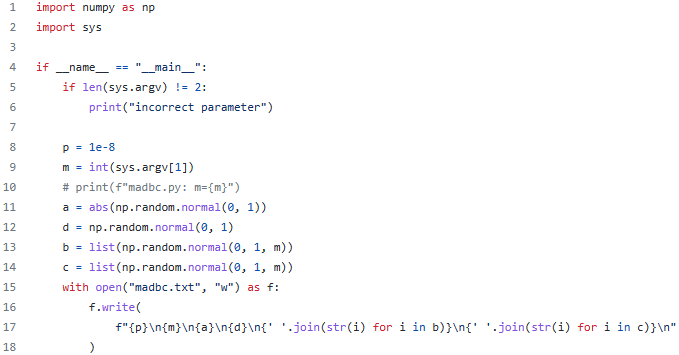
\includegraphics[width=0.5\textwidth]{figures/py@madbc.png}
    \caption{生成测试数据的 Python 程序代码}
    \label{Python}
\end{figure}

测试脚本程序的核心工作是通过调用生成测试数据的 Python 脚本将测试数据写入 madbc.txt,而后调用两个算法程序进行求解,测试脚本的源代码如图 (\ref{Test}) 所示。
\begin{figure}[htb]
    \centering
    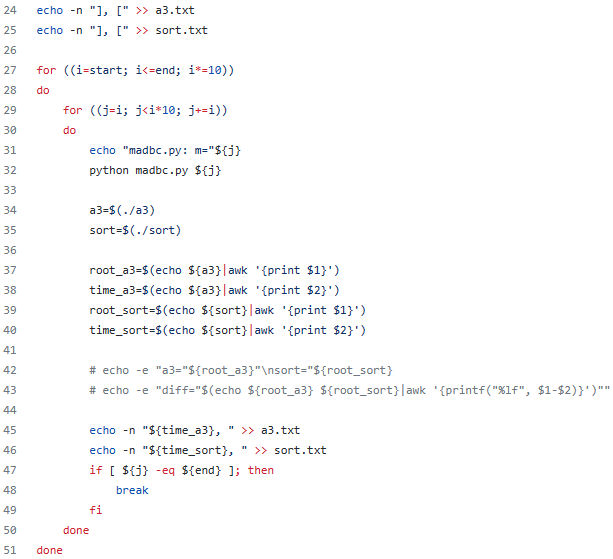
\includegraphics[width=0.5\textwidth]{figures/sh@test.png}
    \caption{测试脚本的源代码}
    \label{Test}
\end{figure}

求解程序通过读入精度、$m,a,d,b,c$ 的值来完成求解,求解完成后将输出求解结果和求解所耗时间,相关的源代码如图 (\ref{Begin}) 所示。
\begin{figure}[htb]
    \centering
    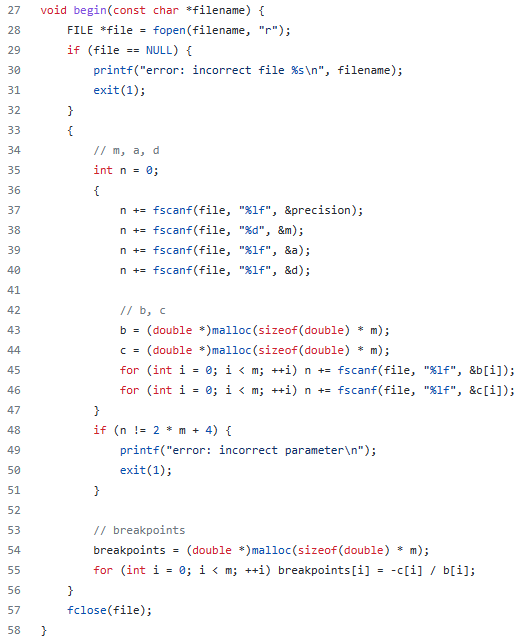
\includegraphics[width=0.5\textwidth]{figures/c@begin().png}
    \caption{求解程序中读取数据的相关源代码}
    \label{Begin}
\end{figure}

\paragraph{图像绘制}

在图像绘制的部分,我们通过使用 Python 语言编写绘图程序,绘制 $10^4$ 个点来对所要求解的函数及函数的次梯度函数进行拟合,绘制的图像可以参考图 (\ref{Answer})。此外,我们还绘制了次梯度函数中每一个分段上的延长线,这样可以更清晰的展示函数中各个分段的关系,便于展示和理解。绘图程序的部分源代码如图 (\ref{Plot}) 所示。
\begin{figure}[htb]
    \centering
    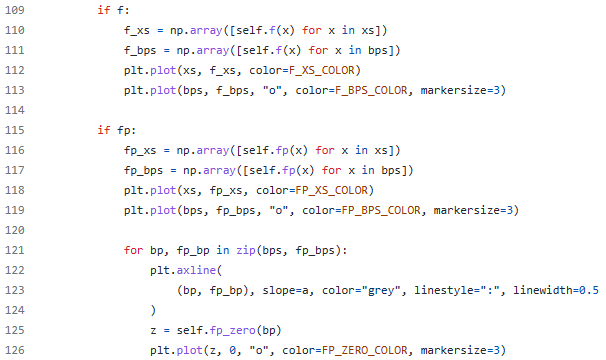
\includegraphics[width=0.5\textwidth]{figures/py@plt.png}
    \caption{绘图程序的部分源代码}
    \label{Plot}
\end{figure}

测试脚本的源代码均已上传至 GitHub 仓库 \href{https://github.com/xqm32/unix-report}{https://github.com/xqm32/unix-report},绘图程序的源代码也已上传至仓库 \href{https://github.com/xqm32/unix-report-python}{https://github.com/xqm32/unix-report-python}。